El propósito del marco teórico es dar un contexto general y clave para todos los lectores. En este apartado se explican conceptos tanto teóricos como contextuales que sean valiosos para la definición del proyecto. De esta forma se da un contexto general incluso para aquellos que no tengan mucha información acerca del tema y puedan interesarse en el proyecto.

Con el marco teórico definido se refleja la  importancia del problema planteado. Su sustento teórico permite entender el problema en su totalidad y crea interés en los lectores. Es así como el marco teórico se presenta de forma jerárquica para ir desarrollando los temas en grado de importancia (los más importantes primero) describiéndolos no solo conceptualmente sino también su relación con el proyecto.

\section{Definición de videojuego}

La definición de un videojuego es bastante variada e incluso ambigua. Según la Real Academia Española, este se define como un dispositivo electrónico que permite, mediante mandos apropiados, simular juegos en la pantalla de un televisor, una computadora u otro dispositivo electrónico \cite{rae2026videojuego}. Jane McGonigal, diseñadora de juegos y escritora estadounidense, describió en su libro Reality is Broken: Why Games Make Us Better and How They Can Change the World una perspectiva más técnica y funcional. McGonigal describe un juego como un sistema que cumple con cuatro pilares fundamentales: un objetivo, reglas, sistema de retroalimentación y acuerdo de participación \cite{mcgonigal2011}.

\begin{figure}[H]
    \centering

    \begin{tikzpicture}[
        pillar/.style={
            rectangle,
            rounded corners=4pt,
            draw,
            thick,
            minimum width=3.2cm,
            minimum height=1.3cm,
            align=center,
            font=\small
        },
        central/.style={
            ellipse,
            draw,
            thick,
            minimum width=3.2cm,
            minimum height=1.5cm,
            align=center,
            font=\small\bfseries
        },
        arrow/.style={
            -{Stealth},
            thick
        }
    ]

        % Sistema central
        \node[central] (game) {Juego\\como sistema};

        % Pilar superior
        \node[pillar, above=1.5cm of game] (objective) {
            \textbf{Objetivo}\\
            Propósito del jugador
        };

        % Pilar derecho
        \node[pillar, right=1.5cm of game] (rules) {
            \textbf{Reglas}\\
            Límites y condiciones
        };

        % Pilar inferior
        \node[pillar, below=1.5cm of game] (feedback) {
            \textbf{Retroalimentación}\\
            Información sobre las acciones
        };

        % Pilar izquierdo
        \node[pillar, left=1.5cm of game] (agreement) {
            \textbf{Acuerdo de}\\
            \textbf{participación}\\
            Aceptación de las condiciones
        };

        % Conexiones
        \draw[arrow] (game) -- (objective);
        \draw[arrow] (game) -- (rules);
        \draw[arrow] (game) -- (feedback);
        \draw[arrow] (game) -- (agreement);

    \end{tikzpicture}

    \caption{Los cuatro pilares fundamentales que caracterizan al juego como sistema.}
    \label{fig:cuatro-pilares-juego}

\end{figure}

Estos componentes permiten estructurar una definición formal y comprender la mecánica operativa de los juegos. El objetivo es un resultado específico que los jugadores buscarán obtener. Por su parte, las reglas marcan límites sobre como los jugadores completan la meta. El sistema de retroalimentación indica a los jugadores que tan cerca están de alcanzar el objetivo. Por último, el acuerdo de participación indica que cada uno de los jugadores del juego está de acuerdo y acepta el objetivo, las reglas y el sistema de retroalimentación del sistema \cite{mcgonigal2011}. 

Al determinar estos elementos indispensables, se establece un estándar de calidad y funcionalidad para el software que será presentado a las diversas poblaciones de estudio. Esta base teórica permite fijar los lineamientos que debe cumplir el producto desarrollado en la presente investigación. De este modo, al comprender los elementos esenciales del medio, se asegura que la solución propuesta no solo opere correctamente a nivel técnico, sino que ofrezca una experiencia interactiva coherente y cumpla con los pilares fundamentales antes descritos.

\section{Desarrollo de software enfocado a juegos}
\subsection{Programación Orientada a Objetos}

En el ámbito del desarrollo de software, los paradigmas de programación definen la metodología y estructura empleada para resolver problemas computacionales. Entre estos, se encuentra la Programación Orientada a Objetos (POO), la cual, de acuerdo a IBM, se fundamenta en la creación de modelos del problema de destino en sus programas \cite{ibm2026spss}. En términos prácticos, este enfoque organiza el código en “objetos”, los cuales actúan como representaciones digitales de entidades del mundo real o componentes abstractos del sistema.

La POO es el estándar predominante en la industria de los videojuegos debido a su capacidad para modelar elementos complejos como personajes, enemigos, escenarios y sistemas del juego de manera estructurada. Su implementación no solo facilita la organización del código y mejora el mantenimiento del código, sino que resulta indispensable para gestionar la densidad de sistemas concurrentes e interdependientes que caracterizan a los videojuegos modernos.

Para el desarrollo del videojuego propuesto, se ha seleccionado la POO como el paradigma principal de diseño. Esta elección permite una definición clara y modular de los componentes del sistema, lo que garantiza una implementación robusta, simplifica las tareas de mantenimiento y asegura la escalabilidad del proyecto ante futuras expansiones.

\subsection{Motores de videojuegos}

Un motor de videojuegos es un entorno de software especializado que integra módulos críticos como renderizado, físicas, audio, animación, entre otros. Esta infraestructura ofrece un entorno unificado que optimiza y simplifica el ciclo de desarrollo en múltiples plataformas \cite{arm2026gamingengine}. En la actualidad, existe una amplia gama de motores, cada uno con características específicas que pueden orientarse hacia géneros particulares o al desarrollo de propósito general.

Al evaluar las alternativas de implementación, el uso de motores de videojuegos suele representar una ventaja competitiva frente al uso de frameworks (como Love2D) o el desarrollo mediante código puro en lenguajes como C++ o Java. Esto se debe a la robustez de las herramientas de edición y depuración que ofrecen plataformas como Unity, Godot, MonoGame o FlatRedBall \cite{microsoft2026dotnetengines}.

\begin{table}[h!]
\centering
\caption{Comparativa de entornos para desarrollo de videojuegos}
\label{tab:motores_comparativa}

\begin{tabularx}{\textwidth}{|>{\raggedright\arraybackslash}p{3.0cm}|
                              >{\centering\arraybackslash}X|
                              >{\centering\arraybackslash}X|
                              >{\centering\arraybackslash}X|}
\hline

\textbf{Criterio} &
\textbf{Godot Engine} &
\textbf{Frameworks (ej. LÖVE2D)} &
\textbf{Código Puro (C++/Java)} \\ \hline

Arquitectura &
Escenas y Nodos &
Bucles orientados a eventos &
Estructura desde cero \\ \hline

Paradigma Principal &
POO / Composición &
Funcional / Scripting &
Imperativo / POO \\ \hline

Pipeline Editor GUI &
Integrado &
Inexistente (requiere externo) &
Inexistente \\ \hline

Curva de Aprendizaje &
Moderada-Baja &
Baja &
Alta \\ \hline

Licencia / Naturaleza &
Open Source (MIT) &
Open Source (zlib) &
N/A \\ \hline

\end{tabularx}

\end{table}

Para el presente proyecto, se ha seleccionado el motor Godot, una herramienta de código abierto (open source) altamente eficiente para la creación de experiencias 2D y 3D. Una de las razones principales de su elección, además de su arquitectura modular, es el uso de GDScript, un lenguaje de programación especializado y optimizado para la lógica interna de este motor \cite{godot2026docs}.

\section{Inteligencias Artificiales generativas}
\subsection{Fundamentos de los modelos generativos}

Un modelo generativo es una arquitectura de aprendizaje automático diseñada para producir nuevos datos que mantienen las propiedades estadísticas y estructurales de su conjunto de entrenamiento \cite{belcic2025generative}. Si bien este tipo de Inteligencia Artificial ha ganado notoriedad pública a través de modelos de lenguaje de gran escala (LLM) como ChatGPT o Gemini, su funcionamiento técnico se basa en la identificación de patrones y distribuciones probabilísticas. A partir de estos hallazgos, el modelo es capaz de sintetizar contenido original en respuesta a las entradas proporcionadas por el usuario \cite{belcic2025generative}.

En el marco de esta investigación, se busca evaluar el potencial de los modelos generativos en tres áreas críticas: la generación de código, la creación de dibujos y la composición musical. Este enfoque permite analizar la capacidad de dichas herramientas para producir contenido funcional y coherente, sometiendo sus respuestas a un proceso de validación técnica. A partir de la producción obtenida de estos modelos, se estructura la versión del videojuego asistida por IA, integrando los resultados generados en el flujo de desarrollo del producto final.

\subsection{Modelos de Lenguaje de Gran Escala (LLMs)}

Los modelos de lenguaje de gran tamaño (LLM, por sus siglas en inglés) representan una categoría avanzada de deep learning entrenada sobre grandes conjuntos de datos. Esta capacidad le permite comprender y generar lenguaje natural, además de producir contenidos técnicos complejos para una amplia gama de tareas \cite{stryker2025llm}. En el ámbito de la generación de código, los LLM constituyen la herramienta estándar, fundamentándose en la arquitectura de red neuronal denominada “Transformer”, la cual destaca por su eficiencia en la gestión de secuencias y su precisión al capturar patrones contextuales en el texto \cite{stryker2025llm}.

La elección de los LLM para esta investigación responde a que representan el estado del arte en la generación automatizada de código. A diferencia de otros modelos predictivos, los LLM poseen la capacidad de generar lógica de programación con un alto nivel de detalle y coherencia estructural. Esto resulta fundamental para recrear las mecánicas del videojuego y analizar cómo el modelo interpreta y desarrolla la experiencia de usuario a través de la implementación de código funcional.

\subsection{GPT-5.6 Luna}

GPT-5.6 Luna es una variante de los modelos de lenguaje GPT-5.6 desarrollados por la empresa OpenAI, desarrollada específicamente para cargas de trabajo de alto volumen y sensibles al costo. OpenAi lo presenta como su modelo más rápido, manteniendo capacidades de razonamiento y soporte para diferentes niveles de esfuerzo de razonamiento \cite{openai_gpt56_luna_2026}. Además, GPT-5.6 Luna se encuentra disponible mediante la API de OpenAI, lo que permite su integración en aplicaciones y sistemas que requieren procesamiento automatizado de lenguaje natural \cite{openai_gpt56_api_2026}.

La inclusión de GPT-5.6 Luna es fundamental para la viabilidad técnica y metodológica de este experimento, donde se requiere la generación dinámica del diseño y mecánicas del juego de gestión de café. La orientación del modelo hacia cargas de trabajo de alto volumen permite considerar su utilización en escenarios donde deben realizarse múltiples solicitudes durante las sesiones experimentales. Asimismo, su menor costo de utilización frente a otros modelos de la misma familia favorece la escalabilidad de la recolección de datos y contribuye a la viabilidad económica del experimento \cite{openai_gpt56_luna_2026,openai_gpt56_api_2026}.

Dentro del diseño experimental 2x2 planteado, este modelo actúa como el motor central del tratamiento experimental correspondiente a la versión del videojuego a la versión del videojuego asistida por inteligencia artificial generativa. De esta manera, el modelo elegido permite implementar una capa de comportamiento basada en modelos de lenguaje, posibilitando la comparación entre una versión del videojuego fundamentada en lógica determinista o tradicional y otra versión que incorpora comportamientos generados dinámicamente mediante inteligencia artificial.

\section{Experiencia de Usuario (UX)}
\subsection{Fundamentos de UX aplicados a videojuegos}

En su obra The Gamer’s Brain: How Neuroscience and UX Can Impact Video Game Design, Celia Hodent define la “Experiencia de Usuario” (UX) como la percepción integral que un individuo desarrolla al interactuar con un producto, ya sea un sitio web, una aplicación o servicio \cite{hodent2018}. Específicamente en el ámbito de los videojuegos, la UX trasciende la interacción directa con el software, abarcando desde la exposición inicial a tráileres y sitios web hasta el proceso de instalación y la navegación en los menús \cite{hodent2018}. Esta disciplina se sustenta en principios cognitivos críticos como la sobrecarga de opciones (tendencia de las personas a sentirse abrumadas cuando se les presentan muchas opciones) o la ley de Jakob, la cual establece que los usuarios prefieren que un sistema funcione de manera análoga a otros que ya conocen \cite{yablonski2026ux}. La aplicación de estos principios en el diseño de videojuegos resulta esencial para optimizar la fluidez y la satisfacción durante el gameplay.

La integración de metodologías de UX en el desarrollo permite ofrecer una experiencia más cohesiva y accesible. Por ejemplo, el mitigar la sobrecarga de opciones, se pueden diseñar interfaces con selecciones jerarquizadas o limitadas; asimismo, la aplicación de la Ley de Jakob sugiere el uso de esquemas de control y entradas (inputs) estandarizados para fomentar la familiaridad inmediata del jugador con la mecánica de juego.

Finalmente, este marco teórico permitirá evaluar la capacidad de la Inteligencia Artificial para interpretar y aplicar conceptos complejos de diseño. El objetivo es determinar si la experiencia del jugador es equivalente en ambas versiones del videojuego, o si una de ellas demuestra una superioridad cualitativa al integrar estos principios de UX de manera más efectiva.

\subsection{Calidad técnica percibida}

La calidad técnica percibida se define como la evaluación subjetiva mediante la cual el usuario juzga la excelencia, idoneidad, sofisticación, coherencia y correcto funcionamiento percibido de un sistema informático.Este concepto se relaciona con la calidad percibida, entendida como el juicio del consumidor o usuario sobre la excelencia de un producto o servicio, y se diferencia de las mediciones objetivas de rendimiento debido a que representa la valoración subjetiva realizada por el usuario \cite{zeithaml1988consumer}. Desde la perspectiva de la experiencia de usuario, esta evaluación también se encuentra vinculada con las percepciones y respuestas de una persona derivadas del uso o de la interacción con un sistema \cite{iso9241_210_2019}.

En el contexto del contenido generado por IA, este concepto comprende la valoración que realiza el jugador sobre la plausibilidad, coherencia contextual, fluidez y consistencia del contenido producido dinámicamente por el sistema. Exactamente, la aparición de información incorrecta o afirmaciones no fundamentadas,comúnmente denominadas como "alucinaciones" en los sistemas generativos, puede afectar la confiabilidad que los usuarios atribuyen a las respuestas generadas \cite{ji2023survey}. Por lo cual, la calidad técnica percibida se centra en la manera en que el usuario interpreta y valora las salidas del sistema en relación con sus expectativas.

La evaluación de esta calidad resulta indispensable para este estudio, ya que la integración de modelos de lenguaje en videojuegos no depende de características técnicas como la longitud de la respuesta generada, sino también de la forma en que los jugadores perciben el comportamiento producido por el sistema. La experiencia de usuario considera aspectos tanto pragmáticos como relacionados con las respuestas y percepciones subjetivas del usuario durante la interacción con un sistema \cite{iso9241_210_2019}. En consecuencia, si aspectos del juego presentan inconsistencias contextuales, repetitividad excesiva o comportamientos inesperados, estos elementos pueden influir negativamente en la valoración del sistema y en la experiencia de interacción. Medir esta dimensión subjetiva permite determinar si el dinamismo y la variabilidad proporcionados por la versión asistida por IA son percibidos como una mejora frente al comportamiento más predecible de la lógica determinista.

Dentro del diseño experimental planteado para el concepto del juego, la calidad técnica percibida opera como una de las variables dependientes utilizadas para contrastar la versión implementada mediante lógica humana con la versión hecha por GPT-5.6 Luna. A través de instrumentos de evaluación posteriores a la interacción, explicadas más adelante, se recopila la percepción de los participantes respecto a la coherencia y consistencia del gameplay. Este procedimiento permite determinar si los usuarios perciben una mejora en la calidad del comportamiento lógico de la versión asistida por IA generativa o si, por el contrario, la variabilidad del contenido generado es interpretada como una disminución de la calidad percibida del videojuego. 

\subsection{Inmersión y Coherencia Lógica}

La inmersión en videojuegos puede entenderse como un estado de absorción en el que la atención del jugador se concentra en la experiencia proporcionada por el entorno virtual, reduciendo temporalmente la atención dirigida hacia estímulos externos. La literatura sobre experiencia de juego distingue diferentes dimensiones relacionadas con este fenómeno, entre ellas la absorción, la presencia y el compromiso del jugador \cite{brown2004presence,jenett2008measuring}.

Esta relación adquiere especial importancia en videojuegos que utilizan contenido generado mediante modelos de lenguaje, debido a que estos pueden producir respuestas variables o inconsistentes con el contexto \cite{ji2023survey}. En el videojuego desarrollado, la inmersión depende de que los clientes reaccionen de manera coherente con el estado del establecimiento y las acciones del jugador. Por ello, se busca determinar si la flexibilidad de la IA generativa mejora la experiencia o si sus posibles inconsistencias afectan negativamente la inmersión.

Para el experimento, la inmersión constituye una variable dependiente utilizada para comparar las condiciones con lógica humana y con comportamiento generado mediante GPT-5.6 Luna. Su evaluación se realizará mediante instrumentos de experiencia de usuario y presencia, complementados con cuestionarios posteriores a la sesión. Asimismo, la coherencia lógica se analizará a partir de la consistencia de los comportamientos y respuestas de los clientes respecto al contexto del juego. 

\section{Sesgos frente a la IA}
\subsection{Fenómeno del "Valle Inquietante" (Uncanny Valley)}

De acuerdo con la periodista e investigadora Rina Caballar, el “valle inquietante” es un concepto acuñado por el profesor Masahiro Mori que describe un fenómeno psicológico particular: a medida que la apariencia de un robot se aproxima a la humana, la respuesta del observador aumenta hasta alcanzar un punto en el que el parecido es casi perfecto, pero no absoluto, provocando una fuerte sensación de repulsión \cite{caballar2024uncanny}. Este fenómeno se manifiesta como un sentimiento profundo de incomodidad, extrañeza o incluso temor, derivado de la sutil discrepancia entre lo artificial y lo biológico \cite{caballar2024uncanny}.

\begin{figure}[H]
    \centering
    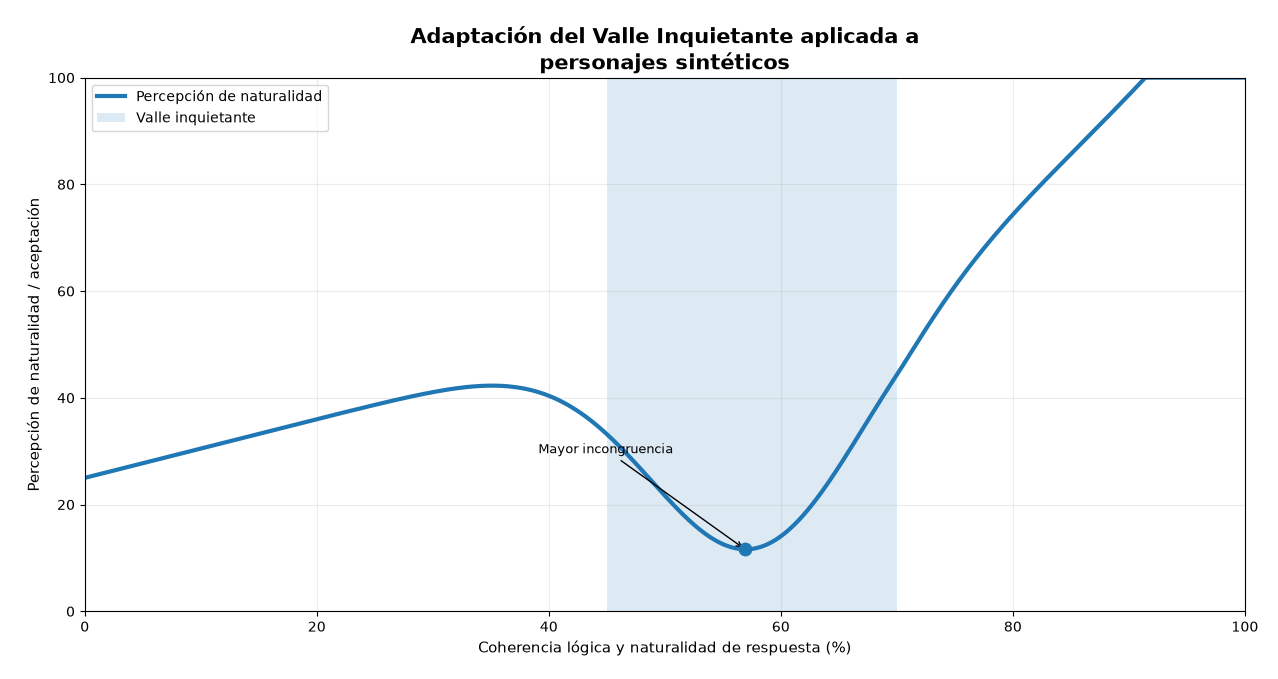
\includegraphics[width=0.8\textwidth]{imagenes/grafica_uncanny_valley.png}
    \caption{Adaptación del Valle Inquietante aplicada a la coherencia lógica y naturalidad de respuesta en personajes sintéticos.}
    \label{fig:valle-inquietante}
\end{figure}

En el contexto de esta investigación, este concepto se erige como un pilar fundamental para explorar la reacción de los usuarios ante la creación artificial. Analizar el valle inquietante permite profundizar en la percepción del contenido generado por IA, identificando los límites donde la simulación tecnológica comienza a generar rechazo en el espectador.

Al exponer a los distintos grupos experimentales a activos generados por IA, será posible monitorear sus respuestas afectivas. Bajo esta premisa, si se observa una reacción de repulsión sistemática hacia la versión asistida por inteligencia artificial, se podría inferir que el contenido ha alcanzado el “valle inquietante”. Esto indicaría que el grado de sofisticación y realismo de la IA ha logrado emular con tal precisión la obra humana que cualquier mínima imperfección es procesada como una anomalía perturbadora por el usuario.

\subsection{Teoría del etiquetado (labeling theory)}

En este ámbito, es posible aplicar principios psicológicos y sociológicos, destacando entre ellos la “teoría del etiquetado”. Esta premisa postula que la desviación de una norma no reside necesariamente en el acto en sí, sino en el hecho de que el individuo pertenece a una minoría, lo que provoca que la mayoría social le asigne automáticamente una etiqueta negativa al alejarse de los estándares comunes \cite{martinez2024etiquetado}. Este fenómeno resulta fundamental para comprender la reacción del público ante el contenido generado mediante Inteligencia Artificial. Dado que los videojuegos se perciben tradicionalmente como un dominio artístico donde la estética y la composición son fruto del esfuerzo humano, el uso de IA suele ser etiquetado de forma prematura como un producto de menor calidad o carente de valor.

Evaluar esta teoría dentro de la investigación permite identificar y analizar los prejuicios preexistentes en las poblaciones de estudio respecto a la versión del juego asistida por IA. De este modo, es posible observar cómo la percepción social predeterminada influye directamente en la valoración técnica y cualitativa de un producto específico.

Debido al desarrollo de dos versiones paralelas del mismo videojuego, se podrá contrastar la validez de la teoría del etiquetado. Al gestionar de forma estratégica la información revelada a los usuarios, se podrá determinar en qué medida el conocimiento sobre el origen del contenido altera la percepción final del producto, permitiendo discernir entre una evaluación objetiva y un sesgo condicionado.


\section{Contexto ético y social de la IA en el desarrollo}
\subsection{Impacto en la industria creativa}

En tiempos recientes, el auge de la inteligencia artificial generativa ha desplazado el debate técnico hacia una esfera ontológica y estética: la disputa sobre si el contenido sintético puede ser legítimamente considerado “arte”. A diferencia de la producción humana, la IA generativa sintetiza nuevos activos a partir de vastos conjuntos de datos preexistentes, lo que ha generado una profunda controversia en las comunidades creativas. La crítica principal radica en que el “arte” algorítmico no se concibe bajo el paradigma de la intencionalidad humana; se argumenta que estas creaciones no emanan de un proceso creativo genuino, sino que son el resultado de un ajuste estadístico de parámetros derivados de un entrenamiento previo \cite{baxter2024aiart}.

Explorar esta transición en la percepción estética resulta fundamental para desarticular las causas del rechazo hacia el contenido sintético. La deshumanización del proceso creativo actúa como un catalizador para el estigma social. Al integrar esta discusión en la investigación, es posible analizar si el juicio del usuario se basa en la calidad intrínseca del activo o en la procedencia del mismo.

Este análisis permitirá determinar si las poblaciones de estudio mantienen una valoración técnica objetiva o si el conocimiento de que el contenido fue generado por una IA le quita valor automáticamente a la obra. En última instancia, se busca comprender si el “aura” del autor humano sigue siendo un requisito indispensable para la validación de un videojuego como producto artístico y cultural. 

\subsection{Reacción de la comunidad y estigmatización}

En años recientes, la integración de la Inteligencia Artificial en el flujo de trabajo de la industria de los videojuegos se ha convertido en una práctica emergente. No obstante, el uso de estas herramientas no es uniforme y su implementación suele generar una reacción adversa en la comunidad de jugadores al hacerse pública. Un caso emblemático es el de Clair Obscur: Expedition 33, un título inicialmente aclamado por su dirección artística; sin embargo, el surgimiento de sospechas o confirmaciones sobre el uso de IA en su desarrollo generó desconfianza entre los usuarios, provocando una pérdida de prestigio dentro del sector \cite{hollyhead2026clair}. Este fenómeno evidencia la consolidación de un estigma que afecta a cualquier producto asociado con procesos generativos automáticos.

Este enfoque permite comprender la arquitectura de la percepción actual dentro de la industria. Analizar las raíces de este rechazo resulta fundamental para identificar estrategias de implementación que permitan utilizar la IA como una herramienta de soporte técnico o creativo sin comprometer la integridad percibida del título ni alienar a la audiencia.

A través de esta comparativa, se evaluará la volatilidad en la percepción del usuario, determinando si la valoración de la calidad del videojuego sufre una degradación significativa al revelar la naturaleza sintética de su desarrollo. En última instancia, se busca discernir si el rechazo es una respuesta a la calidad técnica del producto o una reacción ideológica ante la transparencia sobre el uso de inteligencia artificial.
|

\section{Metodología de encuesta}
\subsection{Pruebas A/B}

Las pruebas A/B consisten en la comparación controlada de dos variantes de un mismo producto para determinar cuál genera una mayor aceptación en la audiencia \cite{oracle2026abtesting}. Este método parte de un modelo base al cual se le modifica una variable específica para observar la respuesta del usuario ante dicho cambio. Aunque su uso es frecuente en el diseño de interfaces web para medir la interacción, su aplicación es igualmente válida para evaluar elementos estructurales en otros medios digitales.

En el presente estudio, se implementan pruebas A/B para contrastar dos versiones de un mismo videojuego: una desarrollada mediante Inteligencia Artificial (IA) y otra mediante métodos tradicionales. Las variables modificadas abarcan el apartado visual (personajes y entornos), sonoro (música y efectos) y, fundamentalmente, el código (mecánicas de gameplay). El análisis se centrará en este último componente, con el objetivo de evaluar la equivalencia y percepción de las mecánicas generadas por IA frente a las desarrolladas de forma convencional.

\subsection{Escala de Likert}

En el ámbito de la medición de percepciones, el instrumento más extendido es la escala de Likert. Se trata de una herramienta psicométrica en la cual el encuestado manifiesta su grado de acuerdo o desacuerdo respecto a un reactivo mediante una escala ordenada y unidimensional \cite{matas2018likert}, permitiendo cuantificar variables subjetivas. No obstante, su efectividad depende del diseño: este método es susceptible a sesgos derivados de la conducta del encuestado y la cantidad de opciones de respuesta, factores que inciden directamente en la calidad de los datos \cite{matas2018likert}.

En esta investigación, dicha escala permite evaluar la percepción sobre el uso de Inteligencia Artificial en el desarrollo de videojuegos. Al contrastar una versión asistida por IA frente a una tradicional, la escala proporciona una métrica determinante para parametrizar el éxito relativo y la preferencia del jugador entre ambas variantes del producto.

\subsection{Players Experience Inventory (PXI)}

El Player Experience Inventory (PXI) es un instrumento psicométrico diseñado específicamente para evaluar la experiencia del jugador en videojuegos. El instrumento organiza la experiencia en diferentes dimensiones relacionadas con aspectos funcionales y psicológicos del juego, permitiendo medir conceptos como inmersión, autonomía, competencia, desafío y control \cite{vermeeren2019pxi}. A diferencia de instrumentos generales de usabilidad, el PXI está orientado específicamente al contexto de los videojuegos y permite evaluar múltiples dimensiones de la experiencia del jugador de manera estandarizada.

La utilización del PXI resulta adecuada para este estudio debido a que permite evaluar los efectos de la incorporación de inteligencia artificial generativa más allá de una valoración general de diversión o satisfacción. Sus diferentes dimensiones permiten analizar si la incorporación de comportamientos generados mediante IA modifica aspectos de la experiencia como la inmersión, el desafío, la autonomía o la percepción de competencia \cite{vermeeren2019pxi}.

Para el estudio, el PXI se utilizará como uno de los principales instrumentos para medir las variables dependientes después de la sesiones de juego. Los resultados obtenidos permitirán comparar la experiencia de los participantes entre la versión con lógica humana y la versión asistida por GPT-5.6 Luna, identificando posibles diferencias en las dimensiones de experiencia evaluadas por el instrumento.